\definecolor{primary}{RGB}{0, 84, 166}
\definecolor{pgold}{RGB}{212, 175, 55}
\definecolor{darkgray}{RGB}{80, 80, 80}

\begin{titlepage}


\begin{tikzpicture}[remember picture, overlay]
    \fill[color=primary!90]
        (current page.north west)
        rectangle ([xshift=0.85cm] current page.south west);
    \fill[color=pgold]
        ([xshift=0.74cm] current page.north west)
        rectangle ([xshift=0.85cm] current page.south west);
    \draw[color=primary, line width=1.8pt]
        ([xshift=1.0cm,  yshift=-2.4cm] current page.north west) --
        ([xshift=-1.2cm, yshift=-2.4cm] current page.north east);
    \draw[color=primary, line width=1.8pt]
        ([xshift=1.0cm,  yshift=2.4cm] current page.south west) --
        ([xshift=-1.2cm, yshift=2.4cm] current page.south east);
    \fill[color=primary!15]
        ([xshift=-3cm, yshift=0cm] current page.south east) --
        ([xshift=0cm,  yshift=0cm] current page.south east) --
        ([xshift=0cm,  yshift=3cm] current page.south east) -- cycle;
\end{tikzpicture}

\begin{center}
\vspace*{0.2cm}

% ----------------------------------------------------------
% SECTION 1 — Trois logos sur une même ligne
% ----------------------------------------------------------
\begin{minipage}[c]{0.28\textwidth}
    \centering
    
\includegraphics[height=2.4cm,keepaspectratio]{Images/logo iset.png}\\[4pt]
    {\scriptsize\bfseries\color{primary}
        Institut Supérieur des\\
        Études Technologiques\\
        de Radès
    }
\end{minipage}
\hfill
\begin{minipage}[c]{0.28\textwidth}
    \centering
    % ↓ Remplacez par votre logo République Tunisienne
    
\includegraphics[height=2.4cm,keepaspectratio]{Images/logo_republique.png}\\[4pt]
    {\scriptsize\bfseries\color{darkgray}
        République Tunisienne
    }
\end{minipage}
\hfill
\begin{minipage}[c]{0.28\textwidth}
    \centering
    
\includegraphics[height=2.4cm,keepaspectratio]{Images/SolidWall.png}\\[4pt]
    {\scriptsize\bfseries\color{primary} SolidWall Consulting}
\end{minipage}

\vspace{0.5cm}
{\color{primary!60}\rule{0.88\textwidth}{0.6pt}}
\vspace{0.4cm}

% ----------------------------------------------------------
% SECTION 2 — Nature du document
% ----------------------------------------------------------
{\large\bfseries\color{darkgray} Rapport de Projet de Fin d'Études}

\vspace{0.15cm}
{\normalsize\color{darkgray} Présenté en vue de l'obtention du diplôme de}

\vspace{0.15cm}
{\large\bfseries\color{primary} Licence Appliquée en Informatique}

\vspace{0.08cm}
{\normalsize\itshape\color{darkgray}
    Spécialité : Développement des Systèmes d'Information
}

% ----------------------------------------------------------
% SECTION 3 — Titre du projet
% ----------------------------------------------------------
\vspace{0.6cm}

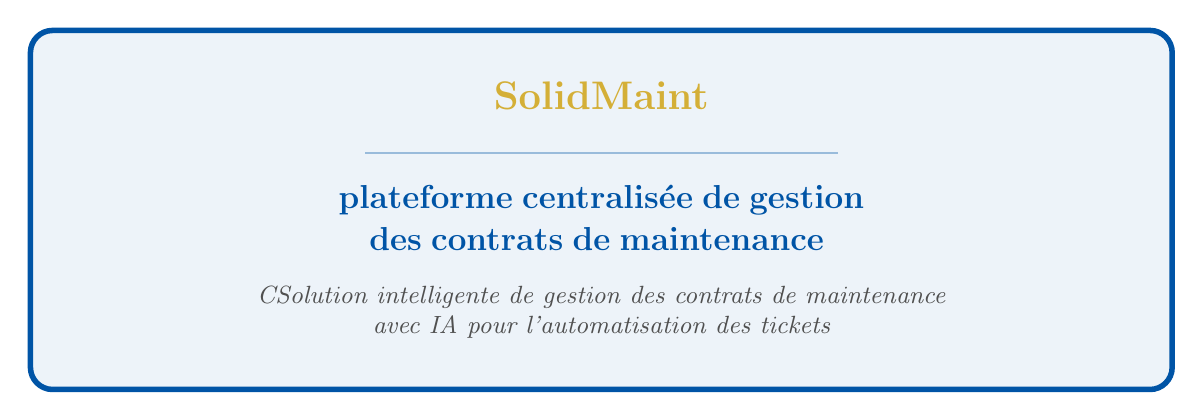
\begin{tikzpicture}
    \node[
        draw          = primary,
        line width    = 2pt,
        fill          = primary!7,
        rounded corners = 8pt,
        inner xsep    = 1.0cm,
        inner ysep    = 0.65cm,
        text width    = 12.5cm,
        align         = center
    ]{
        {\Large\bfseries\textcolor{pgold}{SolidMaint}}\\[4pt]
        \textcolor{primary!40}{\rule{6cm}{0.4pt}}\\[6pt]
        {\large\bfseries\color{primary}
            plateforme centralisée de gestion \\[3pt]
            des contrats de maintenance
        }\\[8pt]
        {\small\itshape\color{darkgray}
            CSolution intelligente de gestion des contrats de maintenance \\
            avec IA pour l’automatisation des tickets\\
            
        }
    };
\end{tikzpicture}

\end{center}

% ----------------------------------------------------------
% SECTION 4 — Réalisé par / Encadré par
% ----------------------------------------------------------
\vspace{0.8cm}

\noindent
\begin{minipage}[t]{0.46\textwidth}
    \raggedright
    \colorbox{primary!12}{%
        \parbox{\dimexpr\linewidth-8pt\relax}{%
            \vspace{5pt}
            \hspace{5pt}{\bfseries\color{primary}\large Réalisé par :}
            \vspace{5pt}
        }%
    }\\[8pt]
    \hspace{8pt}{\large Rihab \textsc{Chourou}}\\[4pt]
    \hspace{8pt}{\large Eya \textsc{Gharbi}}
\end{minipage}
\hfill
\begin{minipage}[t]{0.50\textwidth}
    \raggedright
    \colorbox{primary!12}{%
        \parbox{\dimexpr\linewidth-8pt\relax}{%
            \vspace{5pt}
            \hspace{5pt}{\bfseries\color{primary}\large Encadré par :}
            \vspace{5pt}
        }%
    }\\[8pt]
    \hspace{8pt}{\small\bfseries Encadrante académique : Mme Imen Msekni}\\[2pt]
    \hspace{8pt}{\small\bfseries Encadrante professionnelle : Mme Maissa Ben Fredj}\\[2pt]
\end{minipage}

% ----------------------------------------------------------
% SECTION 5 — Pied de page (taille réduite)
% ----------------------------------------------------------
\vspace*{\fill}

\begin{center}
    {\color{primary}\rule{0.6\textwidth}{0.6pt}}\\[5pt]
    {\small\bfseries\color{darkgray} Année Universitaire 2025--2026}
    \enspace\textcolor{primary!60}{$\vert$}\enspace
    {\footnotesize\color{darkgray} Stage : 02 Fév. -- 31 Mai 2026}
    \enspace\textcolor{primary!60}{$\vert$}\enspace
    {\footnotesize\color{darkgray} Session Juin 2026}
\end{center}

\end{titlepage}